\chapter{METHODS: Motion Correction}
\label{ch:moco}

In the previous chapter, we discuss several techniques used to retrospectively correct motion. Motion correction pipelines may use denoising and filtering, but all pipelines begin with volume registration. In this chapter, we discuss a different approach to volume registration, how it compares to traditional volume registration, and how volume registration fits into a motion correction pipeline. 

%In this section, we discuss the two registration frameworks we apply to our rs-fMRIs: the traditional global volume registration framework and the DAG-based global volume registration framework. The registration frameworks will later be evaluated in comparison to each other, but will also be evaluated in the context of a complete motion correction pipeline. The motion correction pipeline of choice, ICA, will also be discussed in this section.

\section{Directed Acyclic Graph Based Volume Registration}

As discussed previously, the major drawback to Friston et al.'s approach to volume registration is that it only minimized the positional differences between the reference volume and the rest of the sequence. This drawback demonstrates an inability for the traditional approach to account for relationships in the patient's position throughout the scan. Intuitively, we know that the patient's position at any volume in the scan is more similar to his position in the immediately previous or subsequent volume than to another randomly chosen volume in the image.

In our proposed framework, we wish to account for these spatiotemporal relationships between temporally neighboring volumes in the sequence. To accomplish this goal, we start by viewing the rs-fMRI sequence as a directed acyclic graph (DAG). A DAG consists of a set of nodes and edges. Each edge has a direction associated with it and connects a pair of nodes. Since a DAG contains no cycles, there is no possible path back to a node once it has been traversed. 

\begin{figure}
\centering
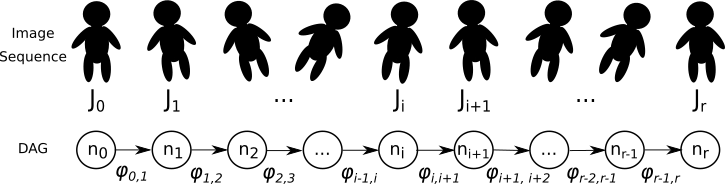
\includegraphics[width=.7\textwidth]{3/dag-chain.png}
\caption{A rs-fMRI can be viewed as a directed acyclic graph where each volume is a node and the edges connect from each volume $i$ to the following volume $i+1$.}
\label{ch3:fig:dag-chain}
\end{figure}

In the case of an rs-fMRI, each volume can be considered a node. The relationship between each pair of temporally neighboring volumes is represented as a directed edge connecting the node for the first volume to the node for the next volume. The acyclic nature of the DAG means that once a patient was in a specific position, he will never return to that exact same position with the exact same neurons firing. The position of the subject and his brain activity as measured by the BOLD signal may be similar in subsequent image volumes, but it will never be precisely the same. The perspectives of an rs-fMRI sequence as a set of images and of the sequence as a DAG can be seen in Figure \ref{ch3:fig:dag-chain}.

The cost of transitioning from one node to the next in our DAG has a parallel representation to the combination of the positional transformation needed to align volume $i$ to volume $i+1$ and the signal change between the volumes. This representation can be written as 

\begin{equation}
J_{i+1} = \phi_{i,i+1} J_i + \delta s_{i,i+1} + \epsilon
\end{equation}

\noindent{where $J_i$ and $J_{i+1}$ are volumes $i$ and $i+1$, $\phi_{i,i+1}$ is a matrix of transformation parameters that must be applied to $J_i$ to achieve the patient’s position in $J_{i+1}$, $\delta s_{i,i+1}$ is the natural change in BOLD signal, and $\epsilon$ is the change in BOLD signal due to motion. Currently, there is no way to estimate the natural change in BOLD signal and the change in BOLD signal due to motion without incorporating additional information about the MRI scanner and the patient that is not included in a rs-fMRI. We simplify our representation of the relationship between two volumes to}

\begin{equation}
J_{i+1} = \phi_{i,i+1} J_i + \epsilon^*
\end{equation}

\noindent{where $\epsilon^*$ is the change in the BOLD signal that cannot be accounted for after aligning the patient’s position in the two volumes. Here, we use the notation $\epsilon^*$ to represent the generic error change in BOLD signal across any pair of volumes.}

After aligning two volumes $i$ and $i+1$, we will then align volumes $i+1$ and $i+2$:

\begin{equation}
\begin{split}
J_{i+2} & = \phi_{i+1,i+2} J_{i+1} + \epsilon^* \\
& = \phi_{i+1,i+2} (\phi_{i,i+1} J_i + \epsilon^*) +\epsilon^*\\
& = \phi_{i+1,i+2} \phi_{i,i+1} J_i + \epsilon^{*'}\\
\end{split}
\end{equation}

\noindent Traditional volume registration assumes that 

\begin{equation}
\phi_{i,i+2} = \phi_{i+1,i+2} \phi_{i,i+1}
\end{equation}

\begin{figure}
\centering
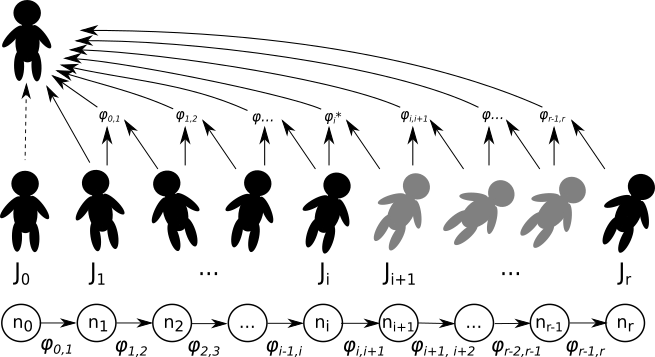
\includegraphics[width=.7\textwidth]{3/dag-registration.png}
\caption{The traditional approach to volume registration in an rs-fMRI sequence consists of registering all volumes in the sequence to a single reference volume.}
\label{ch3:fig:dag-reg}
\end{figure}

\noindent{and calculates $\phi_{i,i+2}$ directly. We argue that this assumption is not true in all cases. Rather than directly calculate $\phi_{0,i}$ and use it to align volume $i$ to the reference volume as the traditional method does, we calculate each component $\phi$ that is a factor of $\phi_{0,i}$. Each component $\phi_{i,i+1}$ is combined with the preceding $\phi_{0,i}$s to recursively align volume $i+1$ to the reference volume without making the large and often inaccurate transformations required by directly calculating $\phi_{0,i+1}$.} This process is outlined in Figure \ref{ch3:fig:dag-reg}.

\section{Independent Component Analysis}

The purpose of image registration is purely to ensure the position of the patient throughout the entire rs-fMRI is consistent. After registration, the image still contains BOLD source signals and noise signals caused by factors other than brain activity. The challenge of separating these combined signals is called blind source separation (BSS). 

We chose to focus on an independent component analysis (ICA) approach for solving the BSS problem. The specific technique we use has been described by Beckmann and Smith as probabilisic ICA. This section aims to provide an overview of the probabilistic ICA technique. For further details, please refer to the technical reports by the FMRIB group \cite{Beckmann2004} \cite{Woolrich2004} \cite{Beckmann} \cite{Smith2004}.

Probabilistic ICA is a linear regression model which performs mixing in the original data space and assumes the true BOLD signal has been confounded by Gaussian noise. These constraints mean that BSS can be solved in three steps:

\begin{enumerate}
\item Estimate a joint subspace consisting of source and noise signals and an noise subspace orthogonal to the joint subspace,
\item Estimate the independent sources in the joint subspace, and 
\item Assess the statistical significance of the independent sources.
\end{enumerate} 

Probabilistic ICA treats the voxel intensity values in every frame of the image sequence as a matrix of $V$ voxels across $n$ time points. For each voxel $v_i \in V$, the observed signal in that voxel can be modeled as

\begin{equation}
\label{ch3:eq:ica01}
\vec{x_i} = A \vec{s_i} + \mu + \vec{\eta_i}
\end{equation}

\noindent This equation allows three different types of signals to contribute to the observed voxel values $\vec{x_i}$ for a given voxel across all $n$ timepoints in the sequence. The first type of signal is a vector of non-Gaussian source signals $\vec{s_i}$ across all $n$ timepoints. The source signals are modulated by mixing matrix $A$ whose shape is the number of time points $n$ by the number of source signals $q$. The second type of signal is an offset denoted by $\mu$. The offset constrains the observed signals to be centered around the mean of all observed signals. The third type of signal $\vec{\eta_i}$ is a vector of noise throughout the duration of the sequence. To summarize, probabilistic ICA explicitly assumes that the observed signal in a given voxel can be divided into non-Gaussian source signals, isotropic Gaussian noise signals, and some offset. This assumption makes it easier to separate a source signal from a noise signal: a noise signal will have a Gaussian distribution while a source signal will not. \textbf{The goal of probabilistic ICA is to identify the source signals, $\vec{s}$.}

With this combination of signals in mind, we can write the covariance matrix of the observed data $x$ as

\begin{equation}
\label{ch3:eq:cov-01}
R_x = \langle x_i x_i^T \rangle = AA^T + \sigma ^2 I
\end{equation}

\noindent where $A$ is the mixing matrix, $\sigma^2$ is the standard deviation of the noise, and $I$ is $n$x$n$ identity matrix. The covariance matrix of the observed data $R_x$ can be calculated, but $A$ and $\sigma^2$ are both unknown. The noisy observed data is transformed with respect to the noise sources using a process called whitening. The whitening with respect to noise enforces the assumption of noise following an isotropic Gaussian distribution with a mean of zero and a standard deviation of $\sigma^2$.

The mixing matrix $A$ can be estimated using maximum likelihood estimation. Beckmann and Smith use singular value decomposition of the observed data $X = U(N\Lambda)^{\frac{1}{2}} V$ to model the estimator of $A$:

\begin{equation}
\hat{A}_{ML} = U_q(\Lambda_q - \sigma ^2 I_q)^{\frac{1}{2}}Q^T
\end{equation}

\noindent where $U_q$ contains the eigenvectors associated with the $q$ largest eigenvalues, $\Lambda_q$ contains the $q$ largest eigenvalues, and $Q$ is a $q$x$q$ orthogonal rotation matrix in the whitened observation space such that $QQ^T = I$. %This estimator assumes that the number of source signals $q$ is known. In a noiseless system, the number of source signals is equivalent to the rank of the covariance matrix of the observed data. However, rs-fMRIs are inherently noisy. In this more general case, the number of sources is more complex to determine. Beckmann and Smith suggest that the number of source signals is the same as the number of eigenvalues of the covariance matrix that violate the ``sphericity assumption of the isotropic Gaussian noise model'' \cite{Beckmann2004}. 
The eigenvectors and eigenvalues can be calculated from $X$, but $\sigma$ and $Q$ remain unknown. As noted earlier, the matrix $Q$ is an orthogonal rotation matrix which, when applied to the whitened data $\tilde{x}$, has the same effect of applying an unmixing matrix to the observed data: 

\begin{equation}
\label{ch3:eq:unmixing-01}
W \vec{x} = Q \tilde{x} = \hat{s}
\end{equation}

\noindent Both matrix-vector multiplications serve to estimate individual source signals $\hat{s}$. The estimated source signals are identified by projecting the whited data $\tilde{x}$ onto each row $r$ of the unmixing matrix $Q$ a total of $q$ times:

\begin{equation}
\hat{s_r} = Q_{r,:} \tilde{x}
\end{equation}

\noindent where the $Q_{r, :}$ represents row $r$ of matrix $Q$.  \textit{(Note: A key assumption in this step is that the rows of the unmixing matrix are mutually orthogonal so that they cover the entire space of signal sources. Additional steps described by Beckmann and Smith can be taken to incoporate prior information about the voxels into this step \cite{Beckmann2004}.)}

At this point, the standard deviation of the noise $\sigma^2$ and the source signals are unknown. We can solve the following system of equations jointly to resolve these two unknown quantities:

\begin{equation}
\hat{s}_{ML} = (\hat{A}^T\hat{A})^{-1}\hat{A}^Tx = \hat{W}x = Q \tilde{x}
\end{equation}

\begin{equation}
\hat{\sigma}_{ML}^2 = \frac{1}{n-q} \sum_{l=q+1}^p \lambda_l .
\end{equation}

Solving these equations is an iterative process. First, the mixing matrix and source signals are estimated. These estimations are used to calculate the corresponding estimator of the standard deviation of the noise. Then, the residual noise $\hat{\eta}_i$ at each voxel $v_i$ is calculated:

\begin{equation}
\label{ch3:eq:res-01}
\hat{\eta}_i = (I - \hat{W}^T\hat{W}) x_i.
\end{equation}

\noindent Recalling from Equation \ref{ch3:eq:ica01} how probabilistic ICA views a signal, Equation \ref{ch3:eq:res-01} becomes: 

\begin{equation}
\hat{\eta}_i = (I - \hat{W}^T\hat{W}) A + (I - \hat{W}^T\hat{W}) \eta
\end{equation}

When the correct number of sources has been identified, the estimated mixing matrix will fully span the source signal space. Then, the residual noise will only be related to the true noise:

\begin{equation}
\hat{\eta}_i = 0 + (I - \hat{W}^T\hat{W}) \eta
\end{equation}

Upon reaching this stage in the probabilistic ICA technique, the source signals have been approximated. The source signals are called spatial independent component maps. Normalizing the values in these maps by the variance of the noise produces $Z$-statistic maps. $Z$-statistic maps can be analyzed to identify voxels with statistically significant activations. These activations are attributed to BOLD signal.

One of the major limitations of ICA is that it is highly data driven. It assumes the dataset contains a sufficiently large number of images, each with a sufficiently large number of voxels. Even assuming an ideal data set, the true value of the mixing matrix is dependent on the observed data \cite{Beckmann2004}. Fluctuations in the data can lead to deviations of the residual noise in certain voxels from the true noise. These deviations can produce \textit{type-I} and \textit{type-II} errors when examining the $Z$-statistic maps to identify statistically significantly activated voxels.
 
Additionally, the developers of probabilistic ICA note that not all noise follows the isotropic Gaussian assumption. Noise based in the patient's physiology is likely to be structured in a way that is non-Gaussian. The non-Gaussian noise signals can still be separated from the BOLD source signals, but only if these noise signals are not highly correlated with the source signals.

\section{Motion Correction Pipeline and Implementation}

Both the traditional and novel volume registration techniques were applied independently to each image from the subject cohorts described in Chapter \ref{ch:data}. After registration, three versions of each image existed: the original BOLD sequence, the sequence modified using traditional volume registration, and the sequence modified using the novel registration method.

The registration algorithms applied to rigid tissue types used affine registration with two degrees of granularity. When applied to soft tissue types (ie, placenta),  three nonlinear transformations with increasing granularities were performed after the affine registrations. The exact parameters used for each volume registration can be seen in Appendix A\ref{appendix:registration-params}. The registration frameworks were implemented in Python using the nipype (Neuroimaging in Python Pipelines and Interfaces) library \cite{Gorgolewski2011}. Volume registration used the ANTs (Advanced Normalization Tools) tools as a backend \cite{Avants2014}.

After performing volume registration to ensure the patient is in the same physical space throughout the image sequence, the image sequence may still contain artifacts due to motion. Our registered sequences underwent motion correction via a well-established motion correction pipeline. We chose to use the independent component analysis (ICA) pipeline outlined by Beckmann and Smith \cite{Beckmann2004}. The motion corrected sequences produced by FMRIB's MELODIC tool were saved alongside the original and registered sequences.  

\section{Evaluating Registered and Motion Corrected Sequences Against Gold Standard Usability Thresholds}

The main goal of motion correction is to reduce the effects of motion on the image so that it is usable. The gold standards for rs-fMRI usability as established by Power et al. are that the FD and DVARs metrics must change less than 0.2 mm and 2.5\% normalized voxel units between at least 50\% of the neighboring volumes. The FD and DVARs metrics between each pair of subsequent image volumes were calculated for the original, registered, and motion corrected sequences. The metrics for each sequence were then compared to the gold standard image usability thresholds. This comparison answers the key question of how each registration framework impacts an established motion correction pipeline.

Additionally, a smaller comparison of the registered sequences was conducted. This comparison evaluates the immediate impact of the registration algorithm on the image sequence. It is highly unlikely that an entire image sequence would meet the Power et al. usability thresholds after only the initial step of a motion correction pipeline, but it is valuable to examine the impact of a volume registration algorithm at each stage of the pipeline. 

\textbf{Implementation.} We calculated the FD and DVARS metrics defined by Power et al. using the FSLMotionOutliers tool \cite{Power2012}. 

